\section{مدل علّی و علّت واقعی}\label{sec:causality}

مساله تشخیص علیت در شاخه‌های مختلف علوم کامپیوتر
(به طور خاص، هوش مصنوعی)
کاربرد دارد. روش‌های متفاوتی برای توصیف علیت ارائه شده‌اند
که به طور خلاصه می‌توانیم آن‌ها را به دو دسته تقسیم کنیم:
روش‌هایی که از مفاهیم منطق مجرد استفاده می‌کنند
(مانند روش
\textit{استدلال غیریکنوای}
گِفنِر در
\cite{geffner1990causal})،
و روش‌هایی که از شبکه‌های بِیزی بدست آمده‌اند
(مانند روش
\textit{علت و اثر}
پرل در
\cite{pearl1999reasoning}).
در روش هالپرن و پرل
(که در دسته دوم قرار می‌گیرد)
تعریف خوبی از علّت واقعی ارائه شده است و
جنبه‌های شهودی اصلی علیت در نظر گرفته شده‌اند.
در ادامه به تعریف مدل علّی
و سپس علیت در این مدل می‌پردازیم.

در ابتدا فرض می‌کنیم که مجموعه‌ای مانند
$X$
از
\textit{متغیرهای تصادفی}
در دست داریم.
مجموعه
(محدود)
مقدارهای ممکن برای هر متغیر مانند
$X_i$
را
\textit{دامنه} $X_i$
می‌نامیم و با
$D(X_i)$
نمایش می‌دهیم
($D(X)$
نیز برای نمایش دامنه مجموعه متغیر
$X$
استفاده می‌شود).
با داشتن مجموعه‌های
$X,Y$
و مقداردهی‌های
$x \in D(X), y \in D(Y)$،
برای نمایش اتحاد
$x$ و $y$
از
$xy$
استفاده می‌کنیم.
با داشتن
$x$،
مقدار یک تک‌متغیر
\LTRfootnote{Singleton}
مانند
$X_i \in X$
را با
$x(X_i)$
نمایش می‌دهیم.

\begin{definition}\label{def:causal-model}
  مدل علّی
  $M$
  یک سه‌تایی به فرم
  $(U,V,F)$
  است که در آن،
  $U$
  مجموعه متغیرهای
  \textit{بیرونی}،
  $V$
  مجموعه متغیرهای
  \textit{درونی}
  و
  $F = \set{F_X \mid X \in V}$
  مجموعه‌ای از توابع به فرم زیر است:
  \[ F_X: D(\Par(X)) \to D(X) \]
  $\Par(X)$
  مجموعه متغیرهای پدر
  $X$
  می‌باشد که مقدار
  $X$
  به مقدار آن‌ها وابسته است.
\end{definition}

به صورت شهودی، متغیرهای بیرونی، عوامل محیطی،
و متغیرهای درونی، ساختار درونی سیستم مورد نظر را
مدل می‌کنند.

\begin{definition}\label{def:causal-world}
  با داشتن مدل علّی
  $M$
  و مقداردهی
  $u$
  برای متغیرهای بیرونی آن،
  زوج
  $(M,u)$
  را یک
  \textit{دنیای علّی}
  می‌نامیم.
\end{definition}

در این گزارش، ما تنها مدل‌های علّی
\textit{بازگشتی}
را بررسی می‌کنیم؛ در مدل‌های بازگشتی،
به ازای یک مقداردهی مانند
$u$
برای متغیرهای بیرونی،
مقدار همه متغیرهای درونی
به صورت یکتا تعیین می‌شود؛
این مقداردهی را با
$Y_M(u)$ (یا اختصارا
$Y(u)$)
نمایش می‌دهیم.

\begin{definition}\label{def:causal-submodel}
  با داشتن مدل علّی
  $M=(U,V,F)$
  و مقداردهی
  $x$
  برای
  $X \in V$،
  \textit{زیرمدل} $M$
  (نسبت به
  $X=x$)
  را با
  $M_{X=x} = (U, V, F_{X=x})$
  نمایش می‌دهیم، که در آن
  \begin{equation*}
    F_{X=x} =
      \set{F_Y \mid Y \in V \setminus X} \cup
      \set{F_{X'} = x(X') \mid X' \in X}
  \end{equation*}
\end{definition}

برای اختصار،
$M_{X=x}$ و $F_{X=x}$
را با
$M_x$ و $F_x$
نمایش می‌دهیم؛ همچنین،
به ازای
$Y \subseteq V$،
$Y_{M_x}(u)$
را به اختصار با
$Y_x(u)$
نمایش می‌دهیم.

\begin{definition}\label{def:causal-network}
  \textit{شبکه علّی}
  برای مدل علّی
  $M=(U,V,F)$،
  به صورت زیر تعریف می‌شود:
  \begin{enumerate}[label=(\alph*)]
    \item به‌ازای هر متغیر در
    $U \cup V$
    یک راس در نظر می‌گیریم.
    \item یال
    $X \to Y$
    را اضافه می‌کنیم اگر و فقط اگر
    مقدار
    $Y$
    به
    $X$
    وابسته باشد
    ($X \in \Par(Y)$).
  \end{enumerate}
\end{definition}

\begin{example}\label{ex:causal-model}
  فرض کنیم دو نفر در یک جنگل هستند
  و می‌خواهند با انداختن یک کبریت روشن،
  جنگل را آتش بزنند.
  دو متغیر بیرونی
  $U_1,U_2$
  را برای نشان دادن قصد نفر اول و دوم
  برای آتش زدن جنگل تعریف می‌کنیم.
  متغیرهای درونی
  $A_1,A_2$
  را برای نشان دادن انداختن کبریت روشن
  توسط نفر اول و دوم در جنگل،
  و متغیر
  $F$
  را نیز برای نشان دادن آتش گرفتن جنگل تعریف می‌کنیم. 

  در این مدل، داریم:
  \begin{align*}
    U & = \set{U_1,U_2} \\
    V & = \set{A_1,A_2,F} \\
    F & :
      F_{A_1}=U_1,\,
      F_{A_2}=U_2,\,
      F_{F}=A_1 \vee A_2
  \end{align*}

  برای این مساله، شبکه علّی به صورت شکل
  \ref{fig:cm-example-network}
  می‌باشد.

  \begin{figure}
  \centering
  \def\W{1.5}
  \def\H{0.8}
  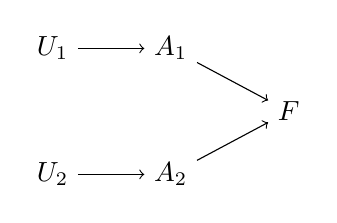
\begin{tikzpicture}
    \node (U1) at (   0, \H) {$U_1$};
    \node (U2) at (   0,-\H) {$U_2$};
    \node (A1) at (  \W, \H) {$A_1$};
    \node (A2) at (  \W,-\H) {$A_2$};
    \node (F)  at (2*\W,  0) {$F$};
    \draw[->] (U1) -- (A1);
    \draw[->] (U2) -- (A2);
    \draw[->] (A1) -- (F);
    \draw[->] (A2) -- (F);
  \end{tikzpicture}
  \caption{
    شبکه علّی برای مثال
    \ref{ex:causal-model}
  }
  \label{fig:cm-example-network}
\end{figure}

\end{example}

با داشتن تعریف‌های بالا،
می‌توانیم مفاهیم علت ضعیف و قوی را توضیح دهیم.

\begin{definition}\label{def:causality}
  با داشتن مدل علّی
  $M=(U,V,F)$،
  مجموعه متغیرهای
  $X$ و $Y$
  و مقداردهی‌های
  $x$ و $y$،
  $X=x$
  یک
  \textit{علت ضعیف}
  برای
  $Y=y$
  در دنیای علّی
  $(M,u)$
  است اگر و فقط اگر شرطهای زیر برقرار باشند:

  \textbf{\lr{AC1}.} $X(u)=x \wedge Y(u)=y$.

  \textbf{\lr{AC2}.}
  مجموعه‌ای مانند
  $W \subseteq V \setminus X$
  و مقداردهی‌های
  $w \in D(W)$ و $\bar{x} \in D(X)$
  وجود داشته باشند، به طوری که:
  \begin{itemize}
    \item[(\lr{a})] $Y_{\bar{x}w} \neq y$.
    \item[(\lr{b})] $Y_{xw}=y$.
    \item[(\lr{c})]
    به ازای هر
    $Z \subseteq V \setminus (X \cup W)$
    به طوری که
    $z = Z(u)$،
    $Y_{xwz}(u)=y$.
  \end{itemize}

  همچنین،
  $X=x$
  یک
  \textit{علت واقعی}
  برای
  $Y=y$
  است اگر و فقط اگر شرط زیر هم برقرار باشد:
  
  \textbf{\lr{AC3}.} $X$
  کمینه باشد؛ در واقع، هیچ زیرمجموعه‌ای از
  $X$
  شرطهای
  \lr{AC1} و \lr{AC2}
  را برآورده نکند.
\end{definition}

در ادبیات علیت، گزاره
$Y=y$
\textit{اثر}
\LTRfootnote{Effect}
نامیده می‌شود.
در ادامه این گزارش، فرض می‌کنیم اثر مورد نظر
یک تک‌متغیر است. این فرض در راستای استفاده ما
از مفهوم علیت است.

\begin{example}\label{ex:causality}
  در سناریوی آتش گرفتن جنگل که در مثال
  \ref{ex:causal-model}
  ارائه شد، با فرض
  $u=(1,1)$،
  $A_1=1$
  علت واقعی
  $F=1$
  است: هر دو گزاره
  $A_1(u)=1$ و $F(u)=1$
  برقرار هستند.
  با تغییر مقدار
  $A_1$ $(\bar{x})$ و $A_2$ $(w)$
  به ۰
  داریم
  $F_{\bar{x}w}(u)=0$.
  واضح است که با بازگرداندن مقدار
  $A_1$ به ۱
  همیشه مقدار
  $F$
  برابر ۱ باقی می‌ماند.
  بنابراین
  $A_1=1$
  دو شرط اول تعریف
  \ref{def:causality}
  را برآورده می‌کند و یک علت ضعیف است؛
  به راحتی می‌توان نشان داد که این مقداردهی
  شرط سوم را نیز برقرار می‌کند،
  و در نتیجه یک علت قوی است.
  به طور مشابه،
  $A_2=1$
  نیز یک علت قوی است.
\end{example}

\textbf{پیچیدگی زمانی مساله علیت:}
آیتر و لوکاسویچ در
\cite{eiter2001complexity}
نشان داده‌اند که با داشتن
$X=x$ و $Y=y$،
مساله
\textit{تصمیم}
علیت
(با علت
$X=x$
و اثر
$Y=y$)
در کلاس پیچیدگی
\lr{$\Sigma_2^P$-Complete}
قرار می‌گیرد. منابع اصلی این پیچیدگی،
جستجو برای
$W$
و بررسی به‌ازای همه مقادیر
$Z$
در شرط دوم، و همچنین بررسی شرط سوم
در تعریف
\ref{def:causality}
می‌باشد.
